\documentclass{dissertation}


\begin{document}

\title{Location Based Multiplayer Mobile Game}
\author{Pedro Henrique de Castro e Melo Carvalho}
\date{April 12, 2021}



\maketitle

%==============================================================================
%% ABSTRACT

\begin{abstract}

Physical exercise, be it walking, running, or cycling, is a vital activity that should be present in the lifestyle 
of the majority of the population and this is a well-known fact, but even still a fair share of the population 
is not engaged in frequent exercise and this is reflected in the obesity problem a lot of countries are facing. 
Additionally, the modern technology industry can serve as a Demotivator for these people with the release of 
countless games, consoles, and other activities that can only be done at home, stimulating a sedentary lifestyle.

Location Based games are not very popular in the gaming industry and although this style of game 
has been explored to great success before (PokemonGo), most apps usually underperform, such as "Harry Potter: 
Wizards Unite" and "Minecraft Earth". This could be attributed to the lack of player-to-player interaction, 
the players aren't visible to each other in any of these games, and although the user can do dungeons and other 
activities with nearby players, they can't actively see the other player on the map, which hinders the multiplayer 
experience.

The concept of this project was to merge the location based game idea, with the idea of a multiplayer game 
where the user can play and interact with friends in real time by having players able to see each other, and 
having one player's action have consequences in the other player's gameplay. Surveys were conducted where 
participants tested both styles of gameplay and answered questions on which style they would be likely to play 
more often and why. It was found that the majority of players find the active multiplayer experience presented 
by this project more attractive than the pseudo multiplayer presented by others.

\end{abstract}

%==============================================================================
%% Educational Consent
\def\consentname {Pedro Henrique de Castro e Melo Carvalho}
\def\consentdate{12 April 2021}

\educationalconsent

%==============================================================================

\tableofcontents

%==============================================================================

\chapter{Introduction}

\pagenumbering{arabic}

This chapter will go through the concepts of location based games, multiplayer games, and how physical 
exercise is treated in the modern days. In addition, the motivation for researching these topics and the 
overall aim of this project will also be explored. The following chapters will go in depth about the background 
behind the project, the requirements that had to be met before starting development, the design of the application, 
the implementation process, how the project was evaluated and lastly, the concluding thoughts.

\section{Motivation}

Physical activity should be present in every capable person's lifestyle. Many studies have been conducted that show 
that physical activity can play an important role in the management of mild-to-moderate mental health illness, such as 
depression and anxiety, for example, aerobic exercises such as jogging, cycling, spinning, etc, can reduce depressive 
symptoms as well as anxiety and panic ones \citep{Paluska12}. In addition to this, even the most basic of physical exercises, 
such as walking, have significant positive impacts on physical health as well. These go from simply reducing body fat and 
increasing muscle strength to reducing the risk of heart diseases and stroke. The most interesting part of all of this is 
that it doesn't need to be a long or demanding exercise, simply walking 30 minutes can already bring many mental and 
physical benefits to an individual's health \citep{Harvard10}.

Most of this information is usually common sense and the large majority of the population is aware of this, but even still 
many developed countries suffer from obesity and mental health crises. Within the UK for example, more than one in five 
people are clinically obese and this an increasing trend, and the number of obese children has tripled in the past 20 years and 
the prediction is that it will continue going up \citep{Shan08}. Similar to this, around one in five people also claim to be 
suffering from depression last year \citep{Wallis21}. Noticing these trends, many companies and individuals have taken 
action and made initiatives to motivate people to take on frequent exercising, and these initiatives are becoming more and 
more technological. These vary from a simple reminder app that reminds the user to exercise daily to whole games based 
on real life activity, which is what this report is going to investigate. The first game that comes to everyone's mind 
when thinking of location tracker games is probably "Pokemon Go", which amassed great success in the months following its 
release, being the most downloaded app in the app store and grossing the highest ever revenue of any mobile game in its 
first month at \$207 million \citep{Iqbal21}. In contrast to PokemonGo, many other apps following the same concept of 
"location based games" were released aiming to have the same success as PokemonGo did, but most of them heavily 
underperformed (specifically "Harry Potter: Wizards Unite" and "Minecraft Earth"), even though the mobile apps industry is 
booming because of the Covid-19 pandemic (the second quarter of 2020 became the largest ever in numbers mobile apps 
downloads and usage) \citep{Perez20}. 

Consequently, the motivation for this project comes from the potential that location based games have as a great motivator for 
physical exercise, as well as a source for entertainment while practising outdoor activities and how companies might be looking 
at this genre, or sub-genre, of game from the wrong perspectives.

\section{Aim}
 
The overall aim of this project is to explore the location based game concept, to investigate if it can be merged with the common 
multiplayer format, and to discover if these two notions work better as a form of entertainment and motivation for users who want to 
implement frequent exercise into their lifestyles. The way to measure this is by having volunteers test out the product for a 
long period of time and measure how long and how often they used the app during the that time.

During this trial period, volunteers were given weekly questionnaires that asked them about play time during the week, 
enjoyment factor, motivation factor, etc. In addition to these trials, quick surveys were also performed in a larger crowd 
to have a better overall grasp of what individuals that would be likely to use these products look for in them, and which 
features they find particularly helpful or unhelpful. This data is then processed and plotted onto graphs using python's 
"matplotlib" library for easy visualization and comparison.

Furthermore, as secondary goal, this project aims to investigate just how efficient (or inefficient) location based games are 
in terms of data usage, real life obstacles such as traffic, and limitations bounded to GPS services.


\chapter{Background}

This chapter will go in depth about what the obesity crisis is and supply statistics and data that show how this crisis is affecting 
the world but more specifically the UK, as well as the history of location based games. In addition to this, this chapter will also examine what is 
the impact of the Covid-19 pandemic on the aforementioned crisis and also on mental health. Furthermore, past papers and researches 
on the subject will be mentioned.

The genres "Augmented Reality Games (AR Games)" and "location based games" are very different in their own rights, but most of the 
more popular games in these genres use both Augmented Reality and Location. Thus, to avoid any confusion this paper won't mention 
any games that use solely Augmented Reality since they're not relevant in this study, and every time the term "AR game" is mentioned 
we will consider that to be referring to games that also rely on location based technology.

\section{Obesity Crisis}

Obesity is a term to describe people whose BMI (Body Mass Index) is above 30 \citep{NHS19}. An individual's BMI can be calculated by 
getting their weight in kg and dividing by their height in metres squared, represented by the formula below \citep{Diabetes21}: 
\[BMI = kg / m^2\]
It is a very common condition in developed countries, and in the UK around 1 in every 4 adults and 1 in every 5 children aged 10 to 11 are obese
 \citep{NHS19}, whereas in the US over 30\% of the population is obese, which is double the percentage of people who were obese in 1968, showing 
that this condition is an increasing trend \citep{Frezza08}. Obesity carries various risks, including type 2 diabetes, coronary heart disease, 
and strokes. In addition to this, obesity is known to affect the individual's quality of life and cause some psychological problems such as depression 
and low self-esteem \citep{NHS19}.

Studies show that this obesity crisis also impact a country's economy directly and indirectly. One of these studies focused on the impact of obesity 
on the United States' state of New Mexico, and it was found that obesity in New Mexico cost around 7300 jobs and thus decreases state and local tax 
revenue by more than \$48 million \citep{Frezza08}. Futhermore, in 2007 diabetes (one of the main consequences of obesity) cost the economy of United States 
around \$166 million in medical expenditures and a stunning \$58 billion in reduced national productivity \citep{Frezza08}. Meanwhile, in the UK, the 
overall cost of obesity to society is around £27 billion, and on top of this the NHS spent an estimated £6 billion on obesity related illness in 2014/15.

Finally, although obesity is such a wide and serious issue, the treatments recommended by NHS are very simple: eat a reduced calorie diet and 
exercise regularly by taking up activities such as walking or jogging \citep{NHS19}. Getting the motivation to start exercising can be a very 
difficult process, but nowadays it is easier than ever thanks to the increasing influence technology has on physical activity. Apps and gadgets can 
serve a great source of motivation through immediate feedback and instant activity analysis such as Nike's "Fuel Band" or the jogging app "Runkeeper" \citep{Bice15}.
Additionally, they can also be a source of entertainment while encouraging exercise, for instance location based games.

\section{Location Based Games}

Location Based Games(LBG) are games that use the player's real time physical position, usually through their device's GPS system. This real-time position 
is then used as an input that has consequences inside the game. The most common way this is used is by having the in game player move accordingly to 
the real life player. Due to the constraints regarding constant GPS access and sometimes constant network connectivity, these games are exclusive for 
portable devices such as smartphones and tablets \citep{Jacob10}.

LBGs are a part of a much broader branch of technology called "Location Based Services" (LBS) which emerged in the early 90s, 
but only became a fast-developing field in the early 2000s which is when Location Based Games started to appear \citep{Huang18}. This was a time when 
people started experimenting with "indie apps" and different art styles for mobile applications \citep{Leorke19} and location based services became more 
mainstream because of the widespread advertisement for GPS technology \citep{Gordon11}.

The first well-known LBG was "Botfighters", a game where players would run around controlling robots that could be killed by nearby players. Once a robot was 
killed, the user would gain some credit that could be used in the game's website for upgrades for their robot \citep{Guardian02}. The game generated a revenue 
of around £35,000 per month, which at the time was considered a success for an independent mobile game \citep{Guardian02}. Following these news, more 
developers changed their focused to this new game genre and many new LBG came into existence, including one of the most successful LBGs to date, "Geocaching". 
However this game doesn't follow the same location based formula as the others, and is essentially a treasure hunt game where players hide real life treasures and later input 
some information regarding that treasure's location, after which other players can then go on a hunt around the area where the treasure was hidden while 
solving riddles to find new clues (See \citep{Geocaching17} for visual explanation). Thanks to this concept "Geocaching" sometimes does not require the mobile device to have 
constant GPS enabled \citep{Jacob10}.

More recently, the LBG genre has stepped into the mainstream with the very popular game "PokemonGo". PokemonGo was released in the summer of 2016 and 
set a world record for app with most downloads in its launch week, and in its first months people were spending more time on it than on Facebook \citep{Techspot19}.
The game was thought to be a viral app that wouldn't last long in the top download charts but as of 2019, the app has been downloaded over a billion times with around 
200 million of those downloads taking place in late 2018 and early 2019 \citep{Techspot19}. Following the great success of PokemonGo, many other games tried to jump on 
the trend, more notably "Harry Potter: Wizards Unite" (which is from the same company as PokemonGo "Niantic"), but didn't have nearly the same success \citep{Verge19}.

\section{Pandemic Impact on Obesity and LBG}

Both of the aforementioned subjects (Obesity and LBG) have been affected by the global Covid-19 pandemic and the subsequential lockdown. A study conducted in Northern Italy 
interviewed people that suffer from obesity a month after lockdown was implemented in the region about how this lockdown impacted their lifestyles, and it was found that each subject gained around 1.5 kg during this month. This was due to the decrease in physical exercise and increase in consumption of unhealthy foods, which could be linked with anxiety/depression caused by solitude during lockdown \citep{Pellegrini20}.

In addition to this, the pandemic has also had an effect on mobile usage, especially on mobile games downloads. A report written on the increase of mobile usage during the 
pandemic has shown that the average global Android user has spent 20\% more time on their mobile device in April 2020 when compared to April 2019 \citep{Sydow20}. 
Furthermore, the number of global monthly game downloads on both iOS and Google Play has increased 20\% during the same period of time \citep{Sydow20}.

On the other hand, this data cannot be applied to Location Based Games as governments disencourage people to go outside, and thus these games have to try new features 
to adapt to the lockdown. The product lead for Pokemon GO has explained that as soon as Covid-19 began to spread in Italy, data pulled from the country showed a decrease 
in walking, which is the main feature of a LBG. To counter this, Pokemon GO's developers have added features to the game that make it so objectives can be achieved with less walking \citep{Francis20}.

\section{Past Research}

This section is going to go through a few research papers and reports that have been made on the subject of Location Based Games and its correlation to physical activity and 
obesity. These papers have been used as a baseline for this report and they explain how location based games came to be and what is their place in the modern day industry.

\subsection{Technology and physical activity motivation}

This paper was written by researchers from the departments of Kinesiology and Sport Sciences and of Exercise Science from the Universities of Nebraska and Colorado in the US. 
It studies how modern technology can serve as a great motivator for people to practice physical activity since they provide instant feedback and entertainment while exercising 
\citep{Bice15}.

It focused on technologies that are solely fitness focused such as the Nike Fuelband and measured "willingness to exercise" by using the Exercise Motivation Inventory-2 (EMI-2) 
method. The authors used this method to obtain quantitative data for "pre-intervention" (without technology) and "post-intervention", the data was then compared against each other
and the results show that after the intervention there was a significant increase in enjoyment for physical activity \citep{Bice15}.

\subsection{A Definition and Brief History of Location-Based Games}

This is a very in depth research into the origins of LBGs written by Dale Leorke from University of Tampere in Finland. It focuses into the first years of location based games, from 
2001 to 2008, and how GPS services were first used as a form of entertainment.

The paper cites and explains the core features from many of the LBG and Alternate Reality Games (ARGs) that started appearing during this initial phase such as the pioneers 
"Botfighters" and "The Beast", and the popular "Geocaching" \citep{Leorke19}. In addition to this, the article also touches on how these first apps serve as a "testbed" for modern 
day LBGs, with many developers trying out innovative features in their games \citep{Leorke19}.

\subsection{Issues in the Development of Location-Based Games}

This paper written by two students at the University of Porto in Portugal is particularly relevant for this report, as it touches on the issues developers may have when creating a 
LBG. The reason these issues are so relevant is because they had to be considered and sometimes dealt with in the development of "Stay Away", they will be further discussed in 
the "Implementation" chapter.

Among the many issues cited by the article, the main ones are hardware limitations; player's fitness and pace; interaction with outside world; and connectivity \citep{Jacob10}, 
all of which also affect "Stay Away". Furthermore, the authors also briefly define the LBG concept and present viable solutions for the issues they found, such as designing the 
game in such a way that forbids players from doing anything that could put them at risk in the real world \citep{Jacob10}.

\section{Summary}

This chapter went through relevant definitions for both Obesity Crisis and Location Based Games, which are two subjects that are considered correlated in this paper. Meaningful 
data was shown for a better understanding of the matter and for easier visualisation. Additionally, this chapter also presented some past research that has been conducted on 
the material and that has served as a starting point for this work.


\chapter{Analysis/Requirements}

\section{Problem Analysis}
The goal of this project was to develop a multiplayer mobile game that uses the location based concept. To achieve this goal we require softwares that enables us to create games, 
retrieve GPS information, and create network connections. Additionally we need to be able to add features to the game that makes it enjoyable to play.

The user must be able to host or join a server and play with multiple other users, furthermore, each player must be able to view other players' positions and movement in-game, in real time. Additionally, walking in real life should have impacts in-game as to encourage physical exercise, it has to be made clear to the player that this is a core mechanic.

\section{Requirements}
The great majority of the requirements were gathered before development started. These requirements come from previous experience with game development and also from 
suggestions provided by the supervisor on the weekly meetings. The requirements have been divided into functional and non-functional for a more organized approach, the core 
difference between these is that functional requirements are about what the app should do, whereas non-functional are about how the system works \citep{Eriksson12}.

Requirements were prioritised using the MoSCoW Prioritasation technique. This technique consists of classifying priorities (requirements) in 4 categories \citep{moscow21}:

\begin{itemize}
	\item \textbf{Must Have}: These are the minimum usable subset of requirements that we guarantee to deliver.
	\item \textbf{Should Have}: These are requirements that are important to the project but not vital.
	\item \textbf{Could Have}: These are requirements that would be desirable to have but are not important.
	\item \textbf{Won't Have This Time}: These are requirements that have been agreed to not be implemented in the current timeframe, but could be part of future plans.
\end{itemize}

The categorization method used in this section is inspired by one used in a student dissertation written by another University of Glasgow Anguel S. Hristozov \citep{Anguel20}. The 
way it works is each requirement will have two labels, the first one is part of the set \{M, S, C, W\} which represent \textbf{Must Have}, \textbf{Should Have}, \textbf{Could Have}, 
\textbf{Won't Have This Time} respectively; the second label is a simple Y or N which mean the requirement has been achieved or not, respectively.

\subsection{Functional Requirements}

\begin{enumerate}
\item \textbf{M - Y}: The user must be able to host or connect to a game lobby within a protected network. This constitutes the multiplayer feature.
\item \textbf{M - Y}: The application must be able to retrieve real time movement from the device. This is necessary in every LBG.
\item \textbf{M - Y}: Users must be able to see each other's movement in real time. This is what will differentiate this game from the likes of Pokemon GO, it will hopefully make the 
game more entertaining and improve re-playability.
\item \textbf{M - Y}: The application must be at least minimally enjoyable. This wouldn't be important if this was a simple application, but since it is a game playability is considered a must.
\item \textbf{M - Y}: Users must be able to play by themselves if they wish to. This feature was particularly relevant during lockdown when the government banned people from doing 
physical exercises together.
\item \textbf{S - Y}: Retrieve the host's IPv4. Important feature that allows the host to share their IP with the other players so that they can join the lobby.
\item \textbf{S - Y}: Have an easy to use UI (User Interface) navigation system. An important feature in every user centreded application.
\item \textbf{S - N}: Players should be able to pause the game to lower chances of a real life accident (e.g. when crossing a road)
\item \textbf{S - N}: Users should be able to connect to a lobby from a public network such as 4G data.
\item \textbf{S - Y}: The game should have textures and sprites for the game objects such as the players and enemies. Art style is very important in games to attract new players \citep{Solarski13}.
\item \textbf{C - Y}: Difficulty System. Allow the host to change between levels of difficulty that would equate to walking, jogging and running.
\item \textbf{C - N}: High Score System. Save the players high score in their device to create a competitive feel and add re-playability to the game.
\item \textbf{C - N}: Soundtrack and/or environment sounds. This would be nice to have in case the players are using headphones. In the other hand users are not encouraged to play 
with headphones on so they will aware of their surroundings.
\item \textbf{C - N}: Different Characters Selection. Merely an aesthetic feature that could be useful when it comes to player distinction, especially when players happen to be very close together.
\item \textbf{C - Y}: Name Input. This is a feature that most games of this genre, if this name is displayed in game it can also serve as a distinction mechanism, similar to character 
selection.
\item \textbf{C - Y}: Customized artwork for the UI, similar to the player and enemy textures, a nice looking UI goes a long way towards attracting players, however this game has very little 
and simplistic UI, so it's not as important.
\item \textbf{W - N}: Allow players to join the same lobby from different places in the real world and have their characters be placed in their own real life position. When players enter the game, the player characters spawn at the same place for everyone and it's only the map that changes, this happens because it would be unbelievably expensive for the game to load the whole world map and load each player exactly where their device is located. Thus the game only properly works if every player in the lobby is in the same place in real life.
\end{enumerate}

\subsection{Non-Functional Requirements}

\begin{enumerate}
\item \textbf{M - Y}: The application must be easily adaptable for future work. At the current time, the game is around 50\% complete and only the core functionalities have been 
implemented. It is paramount that further development can be easily achieved.
\item \textbf{S - N}: Convert the IPv4 to an encrypted integer/ hex. This is necessary for obvious safety issues.
\item \textbf{C - N}: Have an .apk build of the game for USB debugging and also the option to download it from Google Play.
\item \textbf{W - N}: Have players be able to host lobbies from public networks. This is the main issue with the current state of the game, players can only host lobbies using a private Wifi connection, the reason for this is that most public networks such as the device's 3G/4G blocks this kind of access with a firewall for safety concerns. In that case the host would need to 
know their IPv6 and pass it to the other players instead of the IPv4.
\end{enumerate}

\section{Summary}
This chapter went through the main goals for this project and how they could be achieved. Furthermore, this chapter also touched on vital requirements that need to be met so that the 
application works as intended, and also some other minor requirements that would improve security, playability, interaction, etc, but wouldn't break the game if they weren't met.


\chapter{Design}

This chapter will go through the design process of the game as a mobile application. It will present early days wireframes and paper prototypes, explain the architecture of the system and of the server and how the clients communicate with said server whenever they join the game.

\section{Game as Mobile Application}

In this section we will discuss the architecture of the system itself together with the aspects of the user interface.

\subsection{System Architecture}

The architecture for the game system is quite simple in nature and similar to many other games' that follow the "join lobby" formula, below there is a diagram (Figure \textbf{\ref{fig:arch-diag}}
) for the architecture created by the "draw.io" online tool \citep{draw21}.



\begin{figure}[h]
\centering
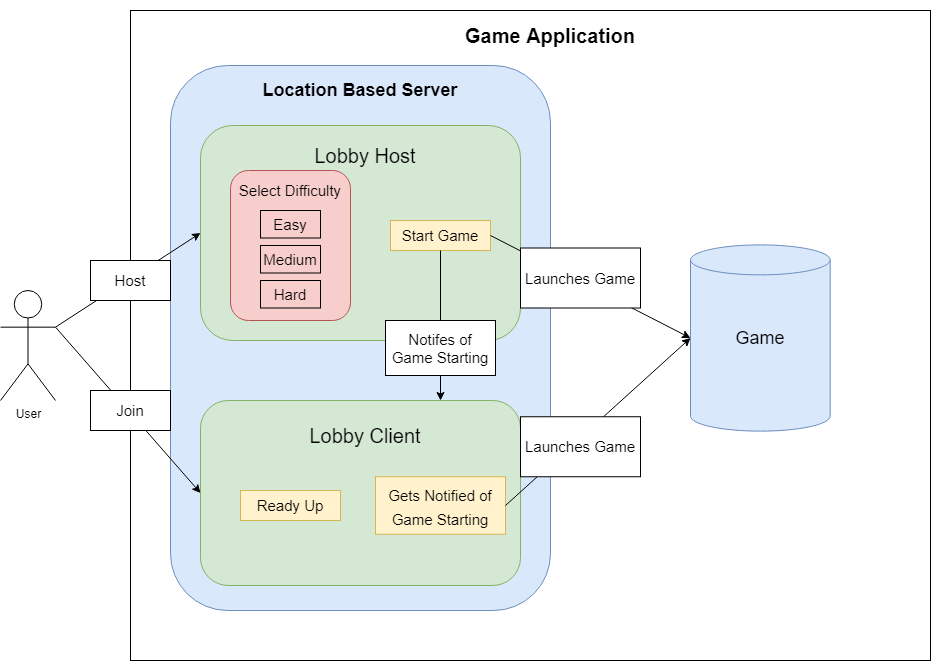
\includegraphics[width = 14cm]{images/system_architecture.png}
\caption{This figure shows the basic architecture of the game as a mobile application. Both the server and the game itself reside in the mobile application which means a user is going to be both server and client.}
\label{fig:arch-diag}
\end{figure}



When users (players) launch the app they can choose between hosting (being a server and client at the same time) or joining an existing lobby, both options connect them to a location based server which will start keeping track of their device's real time position. When in the server, the player has different choices depending if they are a Lobby Host or a Lobby Client. If they are a host they are able to choose the difficulty of the game and also start the game, whereas if they are a client they can simply ready up and wait for the host to notify them of when the game is starting. Once all players are readied up and the host has chosen a difficulty, the game launches on all clients (this includes the host) and people are ready to start playing.

This approach was moulded towards meeting certain "must have" requirements, specifically the functional requirements numbered \textbf{1, 2 and 5}.

\subsection{User Interface Prototypes}

The user interface was created with the requirements in mind. Although there aren't any "must have" requirements regarding the user interface, functional requirement (FR) \textbf{7} shows that having an easy to navigate UI is something the application should have. In addition to this, FR \textbf{15} is also a nice feature that would improve the quality of the game.

The conception for the user interface began very early in development in the form of paper sketches, shown in the figures \textbf{\ref{fig:start-menu} and \ref{fig:lobby-menu}}.

\begin{figure}[H]
\begin{subfigure}[h]{.5\textwidth}
\centering
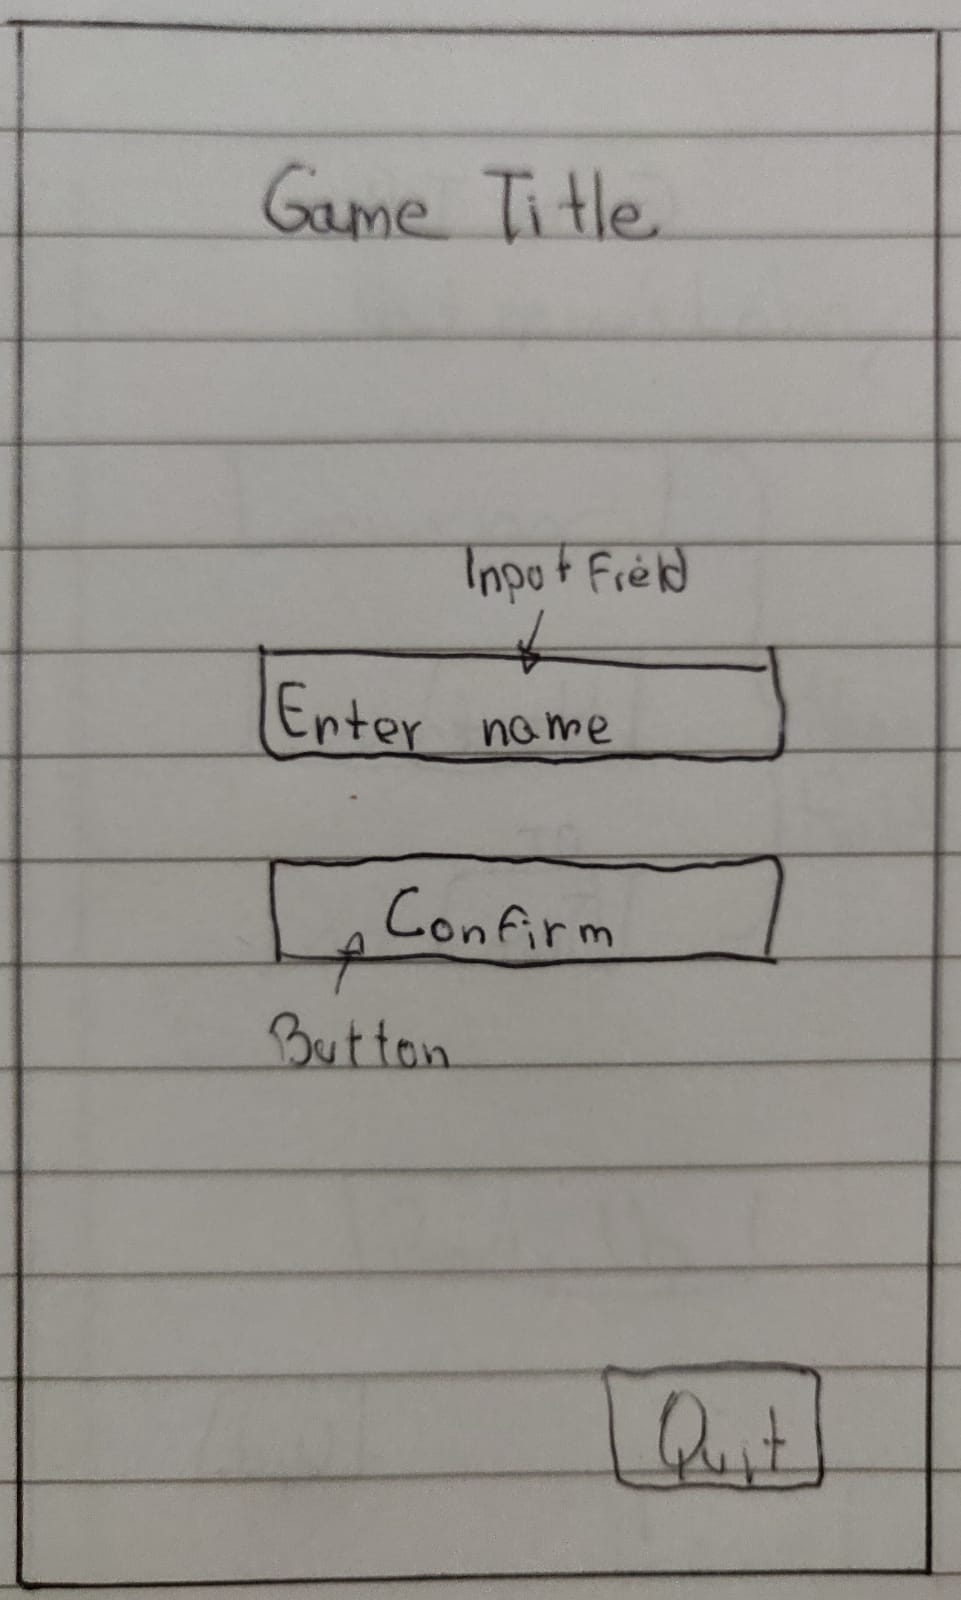
\includegraphics[width = .8\linewidth]{images/paper-prototype1.jpeg}
\caption{Name selection screen}
\label{fig:pp1}
\end{subfigure}
\begin{subfigure}[h]{.5\textwidth}
\centering
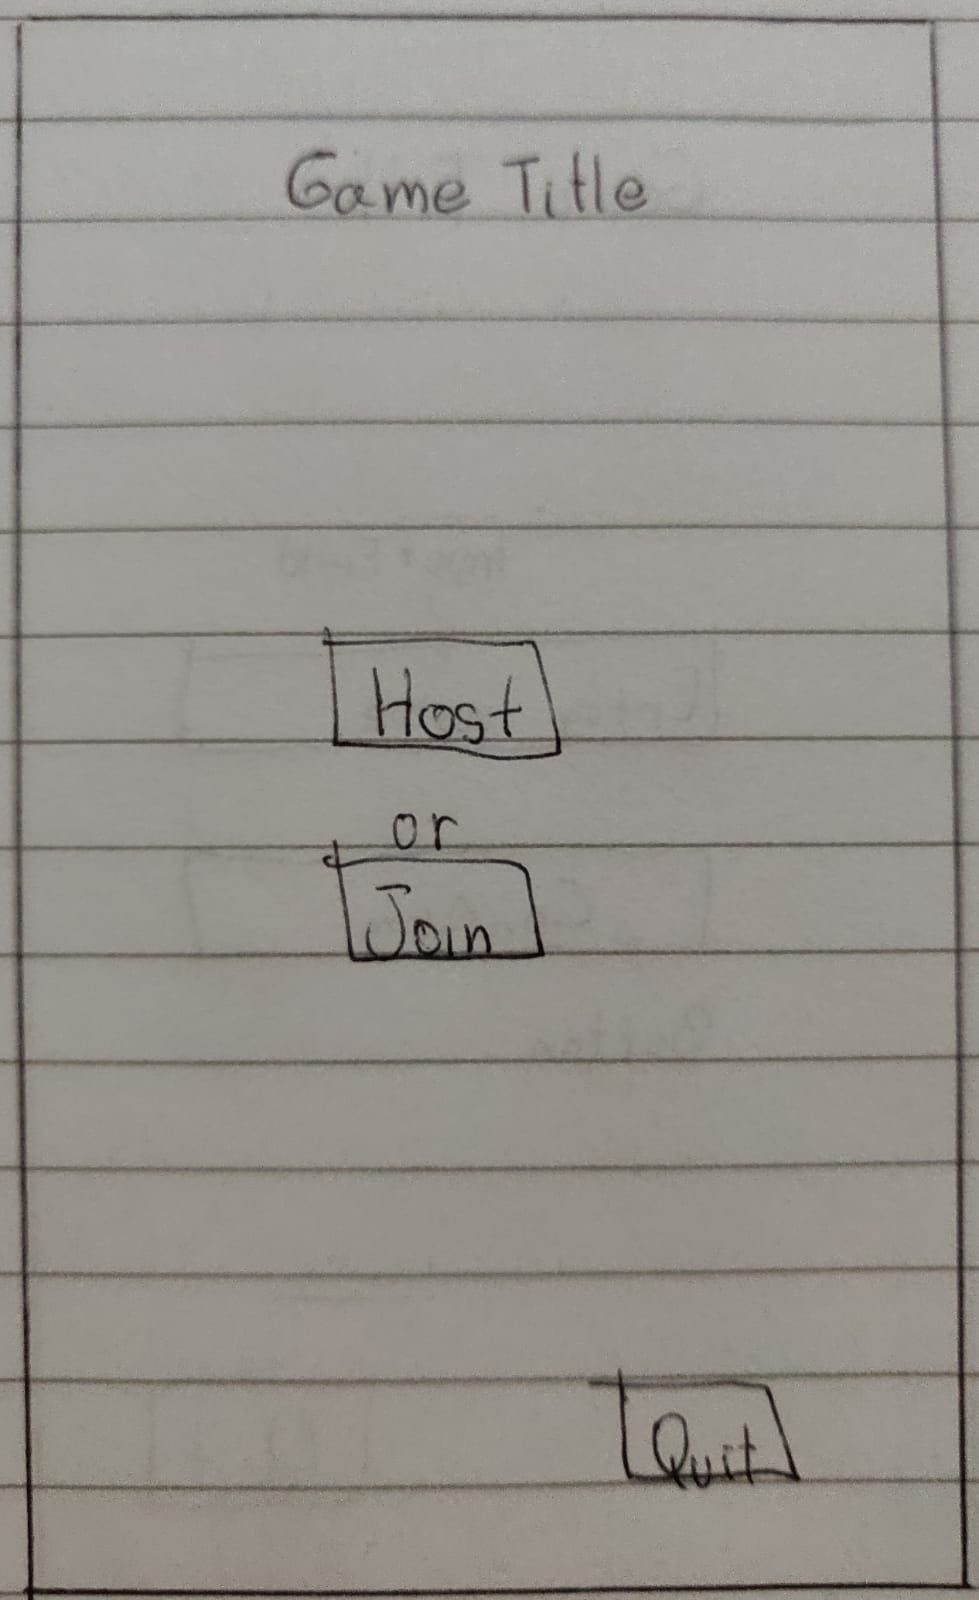
\includegraphics[width = .8\linewidth]{images/paper-prototype2.jpeg}
\caption{Hosting or Joining existing lobby screen}
\label{fig:pp2}
\end{subfigure}
\caption{Paper sketches for the Start menu scene}
\label{fig:start-menu}
\end{figure}

\begin{figure}[H]
\begin{subfigure}[h]{.5\textwidth}
\centering
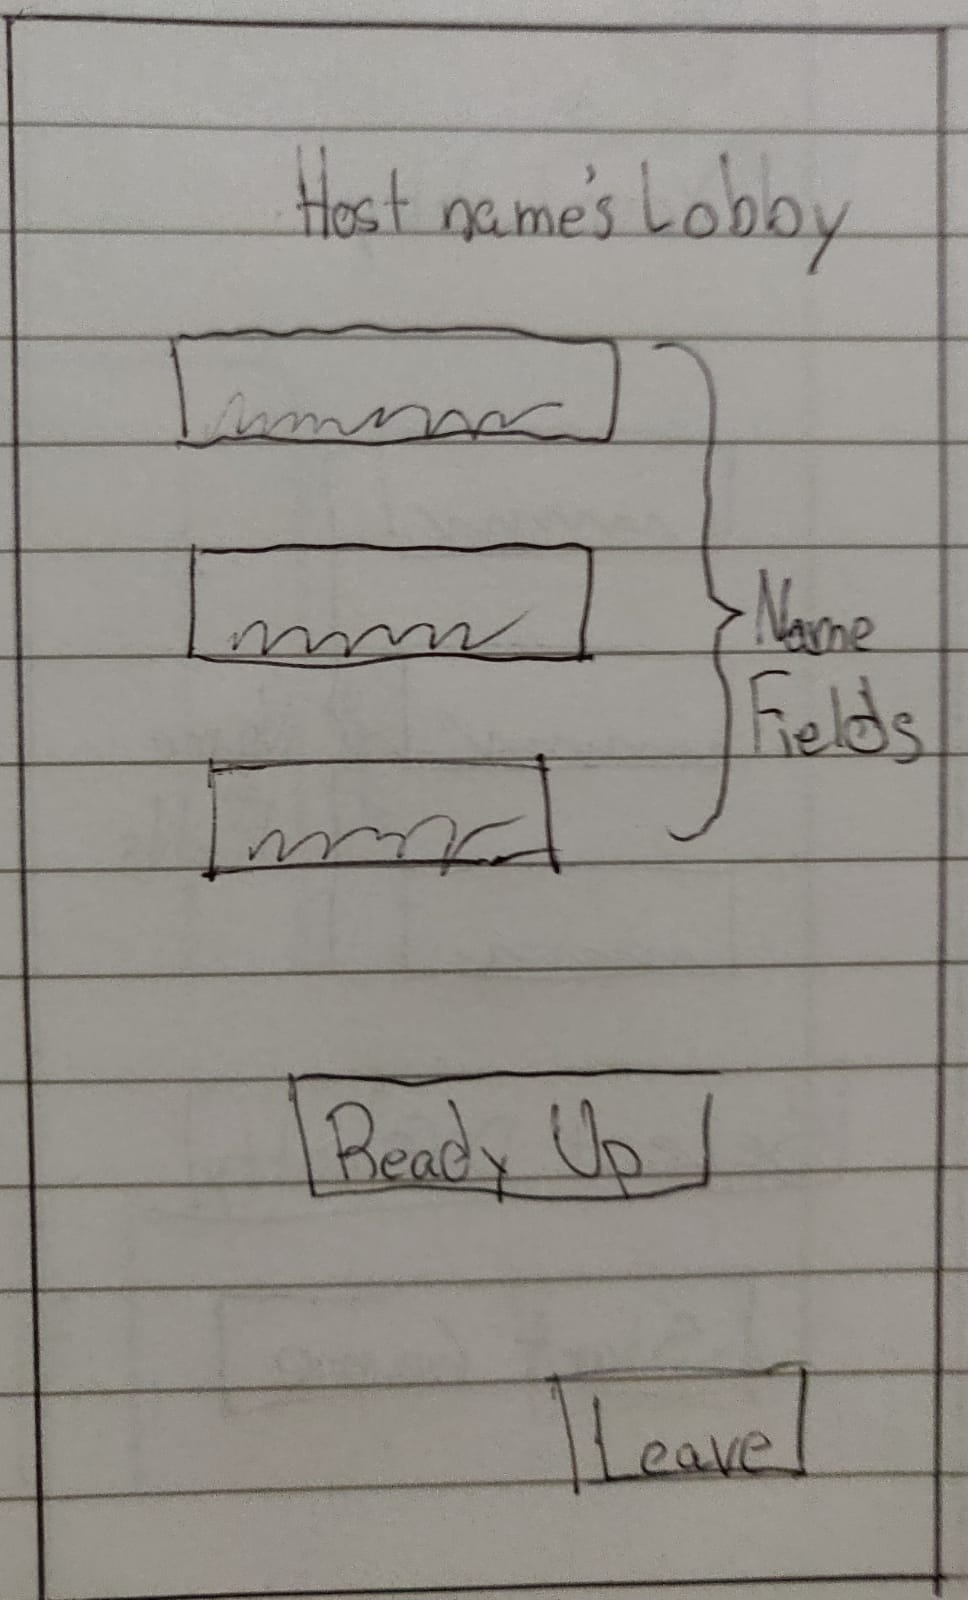
\includegraphics[width = .8\linewidth]{images/paper-prototype3.jpeg}
\caption{Lobby screen for clients}
\label{fig:pp3}
\end{subfigure}
\begin{subfigure}[h]{.5\textwidth}
\centering
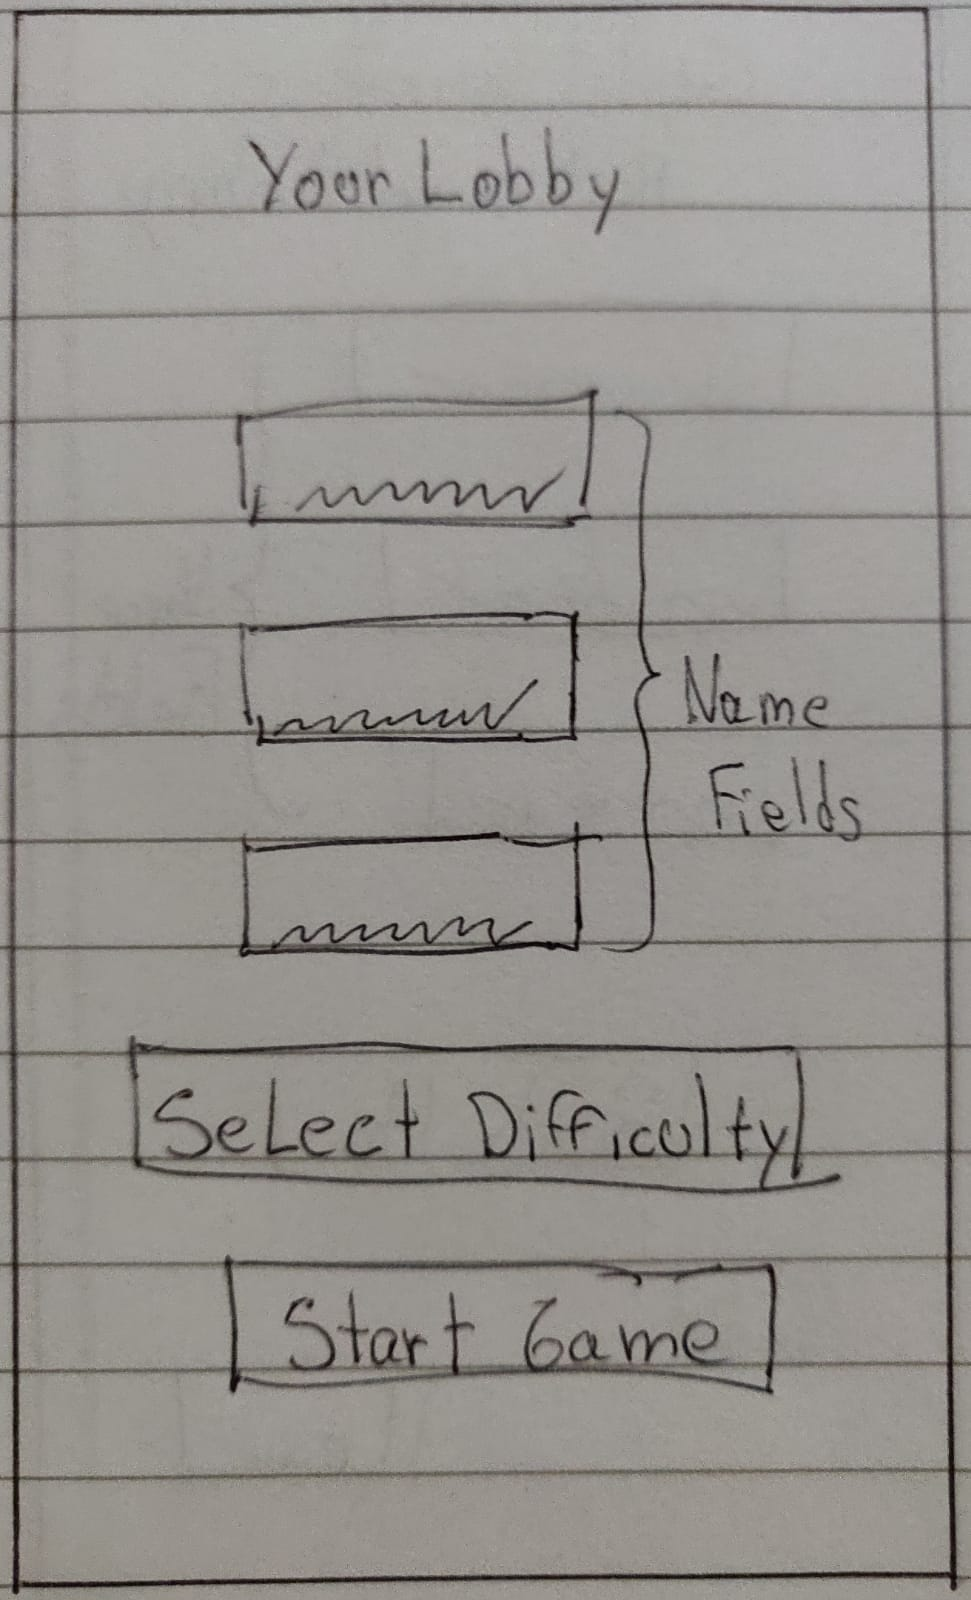
\includegraphics[width = .8\linewidth]{images/paper-prototype4.jpeg}
\caption{Lobby screen for hosts}
\label{fig:pp4}
\end{subfigure}
\caption{Paper sketches for the Lobby scene}
\label{fig:lobby-menu}
\end{figure}

In these figures we can see how the system architecture translates to a user interface. As soon as the user launches the app, they're prompted with a window that asks them to choose the name for their in-game character by using a input field combined with a confirm button, and ideally the software would filter out inappropriate names internally. Once they have entered their name, the user can then choose if they either want to host a lobby in their network or join an existing one.

Moving on to the lobby, the screen should look different depending on if the player is a client or a host, as specified in the system architecture. Although both screens should be able to see the player's names as basic text fields and if they are ready or not, the host screen comes with a "select difficulty" and "start game" button whereas the client screen can only ready up.

\subsection{Initial User Interface}

After the paper prototypes, the next step was to create some more robust and functional wireframes. The wireframes shown in Figure \textbf{\ref{fig:wireframe}} were created using the "Unity" software (also where the whole game was created) and aimed to fulfil virtually every function present in the paper prototypes. 

\begin{figure}[H]
\begin{subfigure}[h]{.5\textwidth}
\centering
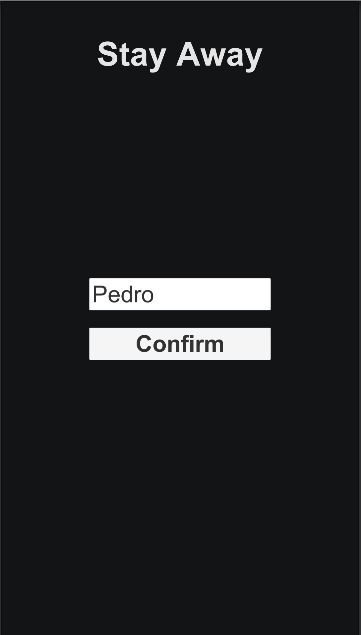
\includegraphics[width = .7\linewidth]{images/wireframe1.png}
\caption{Name selection screen}
\label{fig:pp1}
\end{subfigure}
\begin{subfigure}[h]{.5\textwidth}
\centering
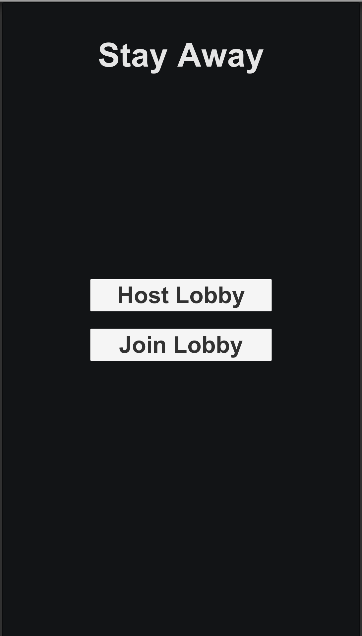
\includegraphics[width = .7\linewidth]{images/wireframe2.png}
\caption{Hosting or Joining existing lobby screen}
\label{fig:pp2}
\end{subfigure}
\begin{subfigure}[h]{.5\textwidth}
\centering
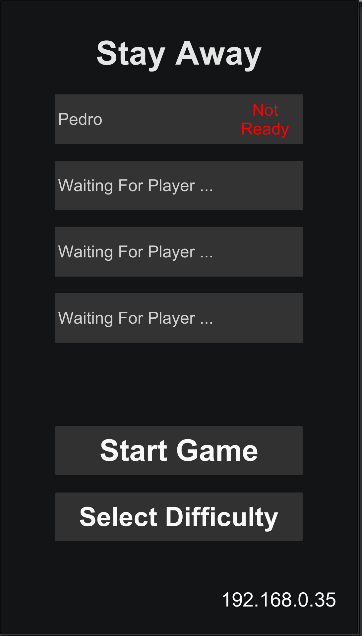
\includegraphics[width = .7\linewidth]{images/wireframe3.png}
\caption{Lobby Screen for Hosts}
\label{fig:pp3}
\end{subfigure}
\caption{Wireframes for user interface}
\label{fig:wireframe}
\end{figure}

These wireframes give a better idea of how the start menu and lobby will look like in-game. Some changes have been made from the previous prototypes, for instance, a "IP address" feature was added which allows players in a lobby to see what IP address that lobby is being hosted on, so they share it with other players. Furthermore, the wireframes didn't include any "Go back/Quit" button which hinders UI navigation, the reason for this is that this testing phase focused more on forward navigation, which is when the user goes downward in the app hierarchy, accessing deeper content \citep{mat21}.

\section{Game Interface}

While creating the paper prototypes for the menu user interface, a prototype for an interface for the game itself was also generated. This interface has been designed to be minimalistic since the game requires the player to have vision of virtually every corner of the screen. 

The paper prototype had 2 buttons, one for settings and one for leaving the game (Figure \textbf{\ref{fig:game-ui}}), but after further consideration, it was decided that the "Leave" button should be included in site the "Settings" one, leaving the screen cleaner. Thus, the only button present in the game interface should be a "settings" button that once clicked enables other buttons for "Leave Game", "Game Settings", "Audio", etc (Figure \textbf{\ref{fig:game-ui2}}).

\begin{figure}[H]
\centering
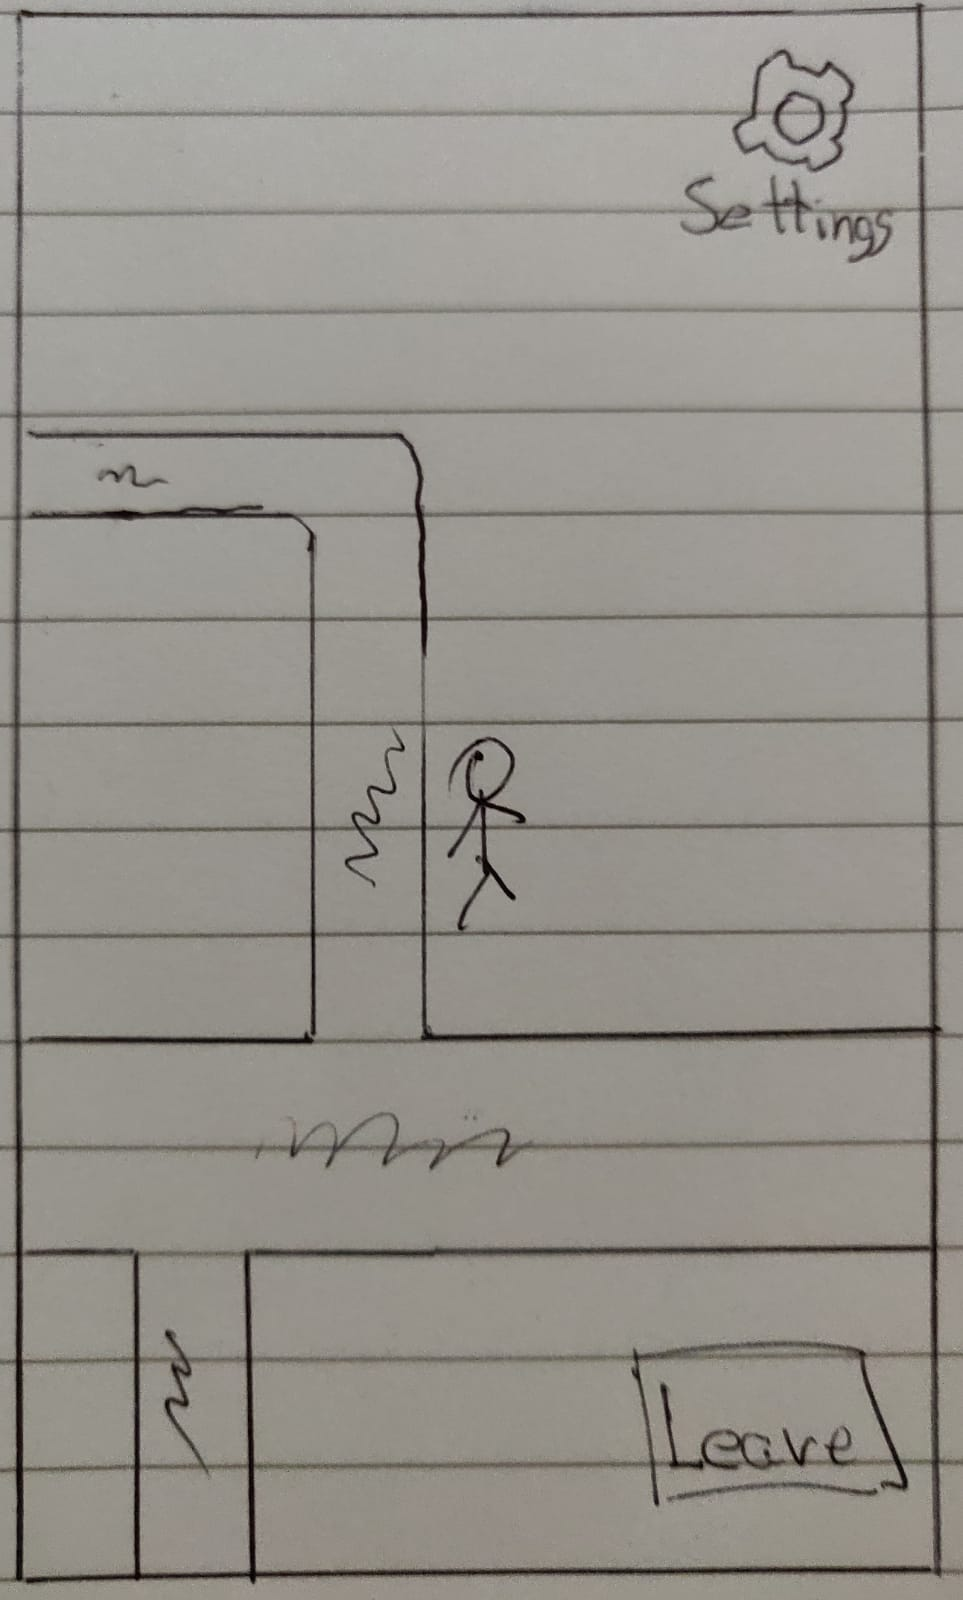
\includegraphics[width = .4\linewidth]{images/paper-prototype5.jpeg}
\caption{This figure shows how the game UI was planned to look like, with a "Settings" and a "Leave" button in the right corners}
\label{fig:game-ui}
\end{figure}

\begin{figure}[H]
\centering
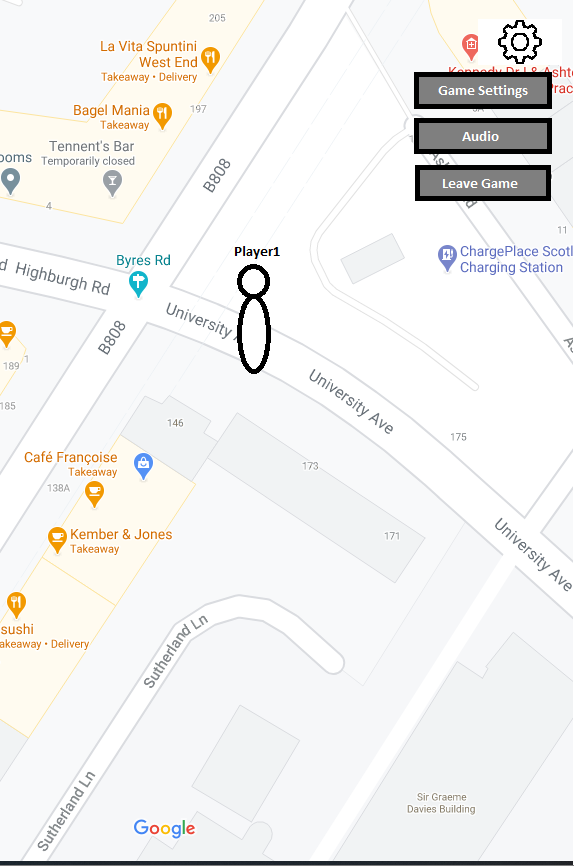
\includegraphics[width = .6\linewidth]{images/game-ui2.png}
\caption{This figure shows how the second iteration of the game UI, with a single "Settings" button that once clicked enables others buttons}
\label{fig:game-ui2}
\end{figure}

\section{Server} 

In early stages we had two options of server architecture to go for. The first one was the well-known "dedicated server" concept, in which the server is hosted in a separate machine or cloud service (AWS, Microsoft Azure) and serves only as a connection and communication point, not operating as a client. The other option, which is the one that end up being used in the project, is the Host architecture, in which a user can choose to host a lobby and operate as both server and client; in this architecture the server is hosted in that user's device and clients connect to that device's IP address as can be seen in the Figure \textbf{\ref{fig:server-arch}}.

\begin{figure}[H]
\centering
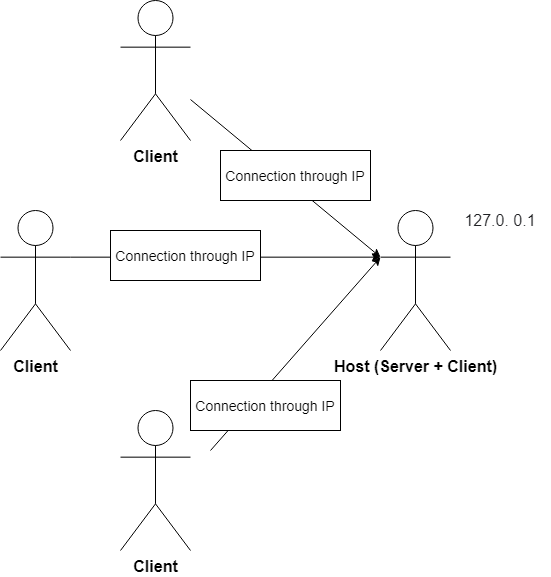
\includegraphics[width = 11cm]{images/server_architecture.png}
\caption{This figure shows the architecture of a LAN server where the server is hosted in a user's device that also acts as a client.}
\label{fig:server-arch}
\end{figure}

This app does not require data that persists from session to session. As a consequence of this, we are able to use Unity's server library that has a built-in database service that helps keep track of persistent data just for that session, which means there will be no need for external database server such as a PostgreSQL server.
\pagebreak

\section{Summary}
 This chapter has gone through the architecture design of several sections of the application. An architecture diagram for the system itself was shown that helps to explain how the functionalities of the system connect with each other. Following this, we presented some initial prototypes for the app's user interface that made use of the architecture diagram, and also some functional wireframes for the user interface. Lastly, a diagram for how clients connect to the server in the app was shown to help explain the "host-client" relation.

\chapter{Implementation}

This chapter will talk over how the designs presented in Chapter 4 have been implemented in the actual game and which tools have been used for that. Furthermore, the chapter will discuss how progress has been tracked for this project and how issues have been dealt with.

\section{Issue and Progress Tracking Process}

In this section we will explore the tools and scripts that were used to help with progress tracking.

\subsection{Version Control}
It was paramount that this project had Version Control. In the first meeting with the supervisor, it was decided that GitHub was going to be tool used for both version control and issue tracking due to its easy-to-use and convenient nature. In addition to this, Git was the version control "language" that I had the most experience with, having work with both GitLab and GitHub in previous projects. 

In the early implementation stages, there were daily commits to the app's GitHub project with the progress done on that day in addition to a progress report. This practice continued for the first 3 months of development but as soon as coding slowed in pace, these commits were done weekly since not a lot (if any) progress was being achieved. The frequent use of Git was proven to be extremely useful for development after a glitch in a software caused the files to be deleted on the PC's hard drive, these files were easily recovered using Git's "pull" feature.

\subsection{Progress Logging}
It was on the guidelines for the project that progress should be logged in a file called "timelog.md" that should be constantly updated, daily if possible; a snippet of how the file looks is shown in Figure \textbf{\ref{fig:timelog-md}}. For more convenience, instead of updating this file manually everyday, a python script that could be executed from command line was created. The python script takes 2 arguments, the amount of hours worked on that particular day and what has been done, the script also retrieves the current date by using the "datetime.today()" function.

\begin{figure}[H]
\centering
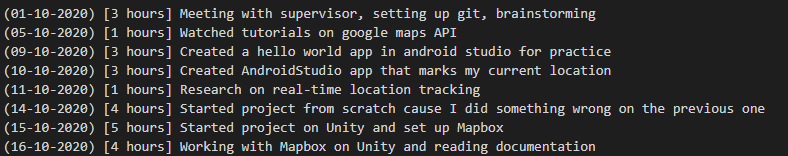
\includegraphics[width = 13cm]{images/timelog-md.png}
\caption{This figure shows a passage from the md file resultant of the timelog script}
\label{fig:timelog-md}
\end{figure}

\subsection{Testing}
This project didn't have any testing mechanisms except for user evaluation. After every modification, the app was transferred from the PC to an Android device to be tested from the eyes of a user. We deemed this testing process to be enough for the game and decided to not adopt any further testing such as CI/CD.

\section{Application}

This section will talk about all the different softwares and libraries that have been used during the implementation of the app.

\subsection{Operating System}
For the mobile operating system, we have chosen to go with Android. There are two main reasons for this, the first is that we had previous experience working with android applications that could be translated into this project, the second is that Android has a greater market share in the UK than iOS devices \citep{Cohen20} (which is where most user evaluations would take place).
The specific Android version that this application was built on is "Android Oreo 8.0" which equates to an API level 26, this version was selected since its apps run on around 60\% of devices while not being outdated.

\begin{figure}[H]
\centering
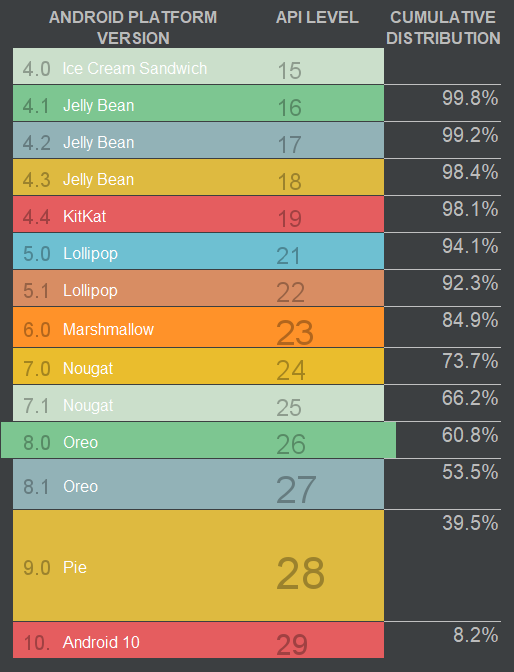
\includegraphics[width = 10cm]{images/android-versions.png}
\caption{This figure shows the percentage of devices that can run apps from each android version, provided by Android Studio}
\label{fig:android-version}
\end{figure}

\subsection{Game Engine}
The game engine of choice for this application was "Unity" \footnote{Getting started with Android development in Unity: \url{https://docs.unity3d.com/560/Documentation/Manual/android-GettingStarted.html}}. We considered a variety of other engines, mainly Android Studio and Xamarin, but Unity ended up trumping other softwares for a variety of reasons. The first and main one, is that we already had previous experience on game developing in Unity (albeit PC games). Secondly, Unity has great cross platform tools, that would enable for the game to be released for both Android and iOS devices with very little alterations \citep{Sinicki20}. Unity also has a large variety of libraries (packages) that would be extremely useful for the development of this project, including many multiplayer support packages and a few location service packages. 

The engine is well-known for it's "visual scripting" that allows for complex operations to take place without the need to code much, but this project focused completely on the use of actual scripting written in the C\# language.

\subsection{Location Service Package}
As mentioned before, Unity has many choices of packages for a lot of different functionalities. Unfortunately location based functionality is not one of those and LBG packages are still somewhat scarce in the platform. Having said that, after some brief research, we found the open-source "Mapbox SDK"\footnote{Mapbox SDK for Unity: \url{https://docs.mapbox.com/unity/maps/guides/}} package which would fit perfectly in this project since it was created with location based games in mind. 

Mapbox became open-source in 2013 but only in 2018 it started being seen as an alternative to the Google Maps API because of the new bigger prices for using such API \citep{Bulatovych19}. Their Unity SDK is quite recent, having been released only in 2017 \citep{Mapbox21}, so there are still some glitches such as having to use an older version of the Unity engine to load some features. 

This package comes with template projects already setup which are super helpful in understanding how the SDK's objects work. For this project we decided to use the "Location-Based game" template as a base to build on top off, this template comes with the map already set up and a yellow player object as can be seen in Figure \textbf{\ref{fig:mapbox-unity}}, this player object follows the user's device real life position.

This service was vital for meeting functional requirements \textbf{2 and 3}

\begin{figure}[H]
\centering
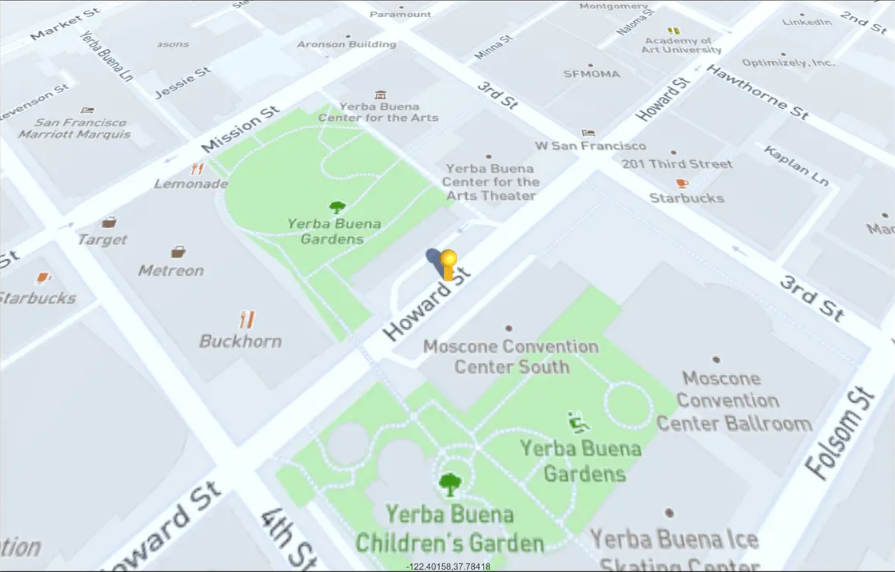
\includegraphics[width = 9cm]{images/mapbox-unity.png}
\caption{This figure shows the template project provided by the Mapbox SDK}
\label{fig:mapbox-unity}
\end{figure}

After having this template setup, the next steps are customizing the objects and map so that it resembles a game and not a navigation app. Mapbox makes it very easy to modify the app to the developer's liking and has a list of open-source user defined maps. For this project we decided to go with a darker map so that it matches the aesthetic of the game a little better (Figure \textbf{\ref{fig:dark-mapbox}}). The last task needed for the package to be completely functional was to integrate it with the multiplayer logic.

\begin{figure}[H]
\centering
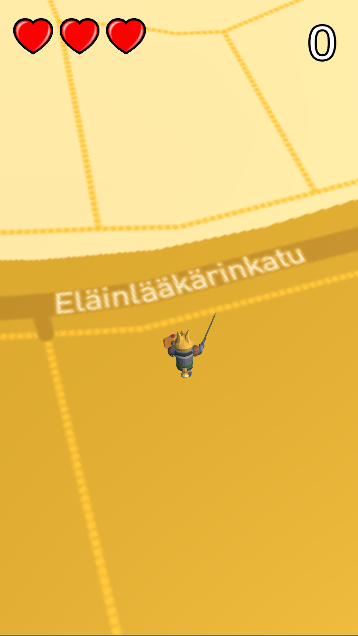
\includegraphics[width = 6cm]{images/dark-mapbox.png}
\caption{This figure shows the map style used in the game}
\label{fig:dark-mapbox}
\end{figure}

\subsection{Multiplayer Logic Package}
For multiplayer support packages we had a diverse set of options but the two main ones that are used by Unity developers is "Photon" and "Mirror". Both of them have been used in successful titles but Photon is a paid service whereas Mirror is free to use, for this reason only we have decided to use Mirror for this project.

Mirror has an extensive documentation \footnote{Mirror Documentation: \url{https://mirror-networking.gitbook.io/docs/}} on its many functions so learning how to work with it wasn't very difficult. In addition to this, there are many tutorials on Youtube that showcase the package and its core features, a tutorial by the youtuber "DapperDino" \footnote{Mirror Youtube Tutorial: \url{https://www.youtube.com/playlist?list=PLS6sInD7ThM1aUDj8lZrF4b4lpvejB2uB}} was particularly helpful with the development of the multiplayer lobby and the syncing of player movement.

This package allowed us to meet functional requirements \textbf{1, 5 and 6}

\subsection{User Interface}
The final user interface didn't stray very far from the paper prototypes in terms of functionality, but some changes were made to its appearance to make it look more like a game UI. 

The first step of improving the appearance of the UI was to choose a color scheme that would be used throughout the whole game. Since the game is supposed to get users to exercise, colours that motivate people's subconsciousness to do physical activity were chosen, such as blue and orange \citep{Elliot15}.

\begin{figure}[H]
\centering
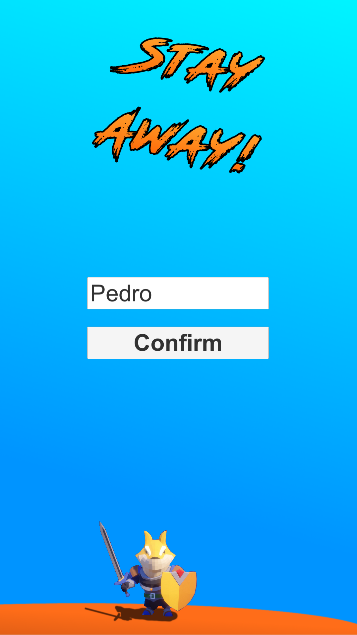
\includegraphics[width = 6cm]{images/final-ui.png}
\caption{This figure shows the start menu UI with an appropriate colour scheme and few buttons}
\label{fig:final-ui}
\end{figure}

Furthermore, the UI is "semi-minimalistic" with very few buttons (Figure \textbf{\ref{fig:final-ui}}) for two main reasons. The first one is that we didn't have previous experience with personalized graphical design but still wanted features in the UI that resembles that of mobiles games. Secondly, a study made in 2019 about minimalism investigated the preferences of users when it comes to UI design, and it was found that the majority of users would rather look at a minimalistic design than a "information-heavy" one \citep{Dong19}.

These choices were made with the intent of meeting requirements \textbf{7, 15 and 16}.

\section{Issues}

This section will discuss the various issues and obstacles faced during the implementation and which of them could not be fixed.

\subsection{Issues with Location Service Logic}
Although setting up the Mapbox SDK package was simple, some issues arrived when implementing custom features. One of these features is having the player character rotate accordingly with the device's rotation, mapbox offers a script that does such thing in one of its templates but when the APK file is built onto the phone for testing, the rotation appears random or not connected to the device. Although it would be a nice addition, this issue couldn't be fixed and is present in the current state of the game.

Furthermore, the way this SDK is coded is not compatible with multiplayer games. Doesn't matter where two players are in the world, if they connect to the same server they will spawn in the same place in game, with both players seeing their own versions of the map location. There is no workaround for this issue and the only "fix" was to provide instructions explaining that for better playability, players should next to each other in real life.

\subsection{Issues with Multiplayer Logic}
Differently from LBG logic that had only one apparent issue, the multiplayer logic provided by Mirror presents a fair amount of major obstacles. The first one regards connecting to a server being hosted from a public network such as 4G data, these networks usually have a firewall blocking these and would require either a proxy or a VPN service to work. If the game had a dedicated server hosted on a cloud server such as AWS' this would not be a problem, but would defeat the purpose of the client-host architecture.

In addition to this, many features that would be desirable in games such as this are not easily achievable with Mirror. The main one is the "Play Again" feature, as soon as a match ends the game over scene would ideally have a play again button that would allow all players to go back to the same lobby and start a new game, but Mirror's Network Manager complicates this. This issue is fixable with more time but won't be present for this iteration.

\section{Summary}
This chapter discussed the technologies choice and also explained how each main element of the application has been implemented. The functional requirements that were met with each implementation were cited. In addition to this, this section also looked at the various issues encountered during the implementation phase.

\chapter{Evaluation}

This chapter will evaluate the implementation methods and discuss what could have been done differently. Following this we will show how the game was rated by study participants and how their feedback helped improve the final product.

\section{Implementation Methods Evaluation}

This section will discuss which implementation methods would have been more efficient than the current ones, and which methods can't be considerably improved.

\subsection{Location Services Implementation}
The implementation of this service followed the best guidelines and the service works almost flawlessly when used in single player, with major issues only appearing when paired with the multiplayer functionality. In addition, the Mapbox SDK is the most widely used and most recommended Location Service for Unity. Thus, there are no obvious improvements to the implementation of this service seeing that most issues are related with the SDK itself and not with how it was implemented, such as the character rotation.

\subsection{Multiplayer Service Implementation}
On the contrairy, the multiplayer service has issues that were caused by how it was implemented. Many of the game glitches that are present in the current build could have been avoided if games were hosted on a dedicated server as opposed to being hosted in a user's device, an attempt to fix this was made in the last iteration but needed more time to be completed. Figure \textbf{\ref{fig:server-lobby}} shows how a lobby hosted on a dedicated server would look like, with a match ID being necessary to join a lobby instead of the IP address.

\begin{figure}[H]
\centering
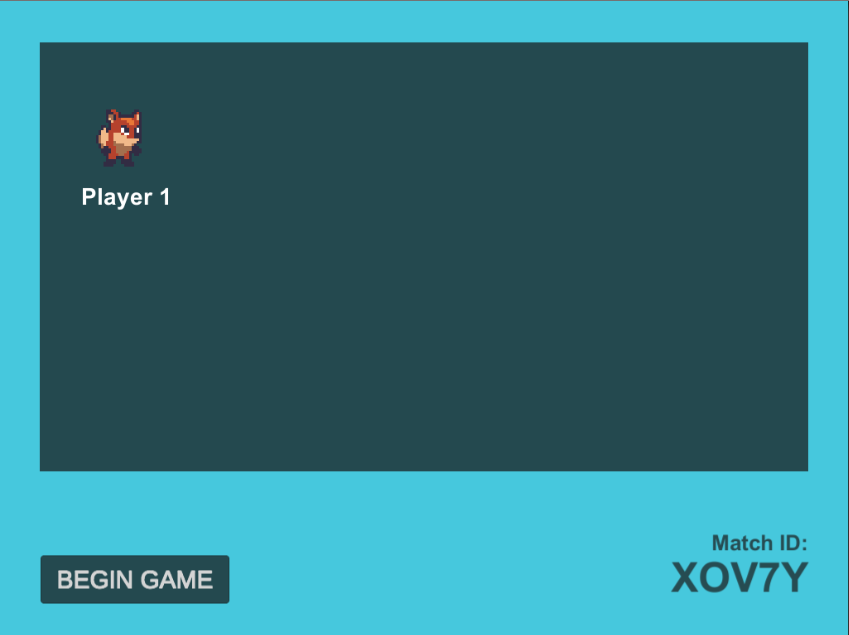
\includegraphics[width = 9cm]{images/ded-server-lobby.png}
\caption{This figure shows a prototype of a lobby that would be hosted in a dedicated server}
\label{fig:server-lobby}
\end{figure}

This implementation would have helped the project meet functional requirements \textbf{9 and 12} in addition to making the implementation of the "Play again" feature much easier.

\section{User Evaluations}

This section will discuss how the product was evaluated by other users and how these evaluations were used to improve the quality of the game. First the methodology used for the evaluation will be discussed followed by the evaluations. In addition to this we will evaluate the project itself by discussing the validation of requirements.

\subsection{Evaluation Methodology}
The application was evaluated by users in two main experiments. The aim of these experiments was to receive feedback on various features of the "Stay Away!" application, this feedback would then be used to improve said application.

\textbf{Experiment 1}

The first experiment consisted of creating a separate Unity application that contained only the User Interface without the actual game. The idea behind this choice was to have users focus solely on the UI so that their responses aren't influenced in any way by the other elements of the application. After testing the application, participants were asked to complete a form on the appearance and feel of the UI.

\textbf{Experiment 2}

The second experiment is similar to the first one, but instead of testing just the user interface they'll test the application as a whole. In this experiment the participants will play the game in real life situations (not on the PC build) so that they have experience a realistic gameplay. The participants were then asked to complete a form on the core game mechanics and were also asked to give suggestions on what would make the game better or more motivating.

\subsection{Pilot Study}
Before conducting the said user evaluation, a pilot study where one chosen participant tested both the user interface and the game has been carried out. The goal of the pilot study was to have a user that is not the developer give a detailed feedback from a user's view and also help identify any underlying bugs before the application was handed out for the main user evaluation. Furthermore, it also helped construct the form with relevant questions that came up during the pilot study.

This study identified a few bugs that were fixed before the main evaluation, for instance, there wasn't a button to leave the credits or instructions screen so the user was stuck there and had to restart the app, these buttons were then added. In addition to this the participant also noted that the game was extremely easy even on the hardest difficulty, thus some variables were changed to make enemies a bit faster and also spawn more often.

\subsection{Results}
\textbf{Experiment 1}

The user interface was evaluated by having users test it on their android phones. This particular form (\textbf{Figure \ref{fig:ui-form}}) was completed by 13 participants that were sent an .APK build to upload to their android devices, these participants were asked 4 questions about what they thought about the UI. These questions were: 

\begin{enumerate}
\item How intuitive was the user interface?
\item How pleasing was the colour scheme?
\item Was it easy to navigate from one page to another?
\item Was the user interface "information heavy"?
\end{enumerate}

The response type was a linear rating scale ranging from 1 to 5, with 1 being the most negative reaction and 5 being the most positive one. The results from this evaluation can be seen on Table \ref{table:1}:

\begin{table}
\begin{center}
\begin{tabular}{ c || c | c | c | c | c  }
\hline 
\textbf{Question} & \textbf{\% Rating 1} & \textbf{\% Rating 2} & \textbf{\% Rating 3} & \textbf{\% Rating 4} & \textbf{\% Rating 5} \\ [0.5 ex]
\hline
1 & 0 & 0 & 23 & 31 & 46 \\
\hline
2 & 0 & 0 & 8 & 31 & 61\\
\hline
3 & 15 & 15 & 15 & 39 & 15\\
\hline
4 & 0 & 0 & 0 & 31 & 69\\
\hline
\end{tabular}
\caption{This table shows the percentage of respondents that gave each rating to the form questions}
\label{table:1}
\end{center}
\end{table}

The general response for questions \textbf{1, 2 and 4} were mostly positive with around 70-100\% of participants rating them with a 4 or 5, thus these features were deemed acceptable and were not improved any further. On the other hand, the responses for \textbf{3} were very mixed and nearly 50\% of participants gave it a rating of 3 or less, meaning that some changes had to be made about navigation. The simple solution was to add backwards navigation so that users can go back and change their name \textbf{Figure \ref{fig:back-button}}, this feature wasn't present before as can be seen on \textbf{Figure \ref{fig:wireframe}}.

\begin{figure}[H]
\centering
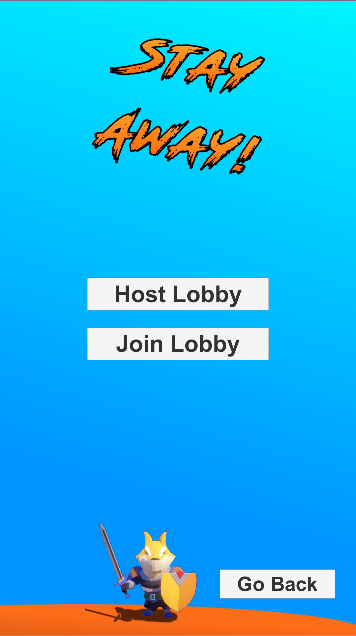
\includegraphics[width = 6cm]{images/back-button.png}
\caption{This figure shows the second screen in the start menu with a "Go Back" button that redirects the user to the name input screen}
\label{fig:back-button}
\end{figure}

\textbf{Experiment 2}

The game mechanics evaluation was conducted by 10 participants that were also sent a .APK file with the whole product that they in turn uploaded to their devices. Unlike Experiment 1 which focused mainly on the aesthetic side, this evaluation's goal was to receive feedback on how the application runs on different systems and how players would view the application. The evaluation form (\textbf{Figure \ref{fig:gf1} and \ref{fig:gf2}}) asked the user for information about their device (what brand, what android version, etc..) in addition to questions about the game itself (is it motivating, is it enjoyable, etc...). The results have been plotted in various charts created using Python's matplotlib \footnote{Matplotlib library: \url{https://matplotlib.org/}}library for easier visualization. 

On \textbf{Figure \ref{fig:android-version-chart}} we can see that the great majority of participants have an android version of 10 or greater, although 10\% were using an android version 8, thus although the target version of the app is 10.0, it was decided to maintain support of earlier versions.

\begin{figure}[H]
\centering
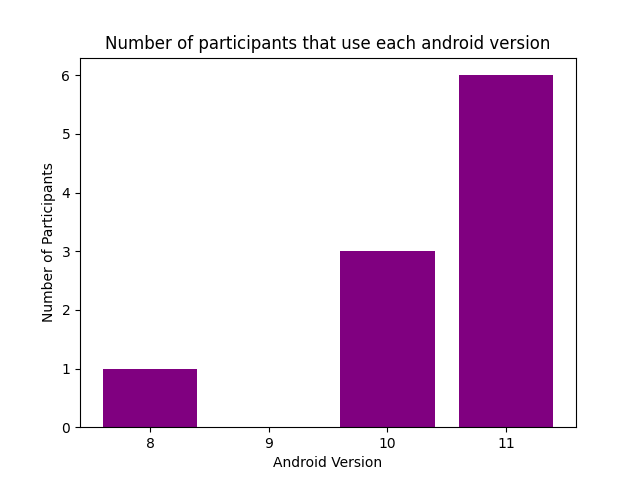
\includegraphics[width = 12cm]{images/android-version-chart.png}
\caption{This figure shows a bar chart created with matplotlib that shows which android versions are more prominent among participants}
\label{fig:android-version-chart}
\end{figure}

Regarding the game mechanics evaluations, the form offered very valuable feedback on what to improve and what to leave as it is. Firstly, although 100\% of the participants played the game on a public setting (Regular Street or Park), only 20\% of them felt the game was unsafe because of traffic accidents as can be seen on \textbf{Figure \ref{fig:unsafe-chart}}.

\begin{figure}[H]
\centering
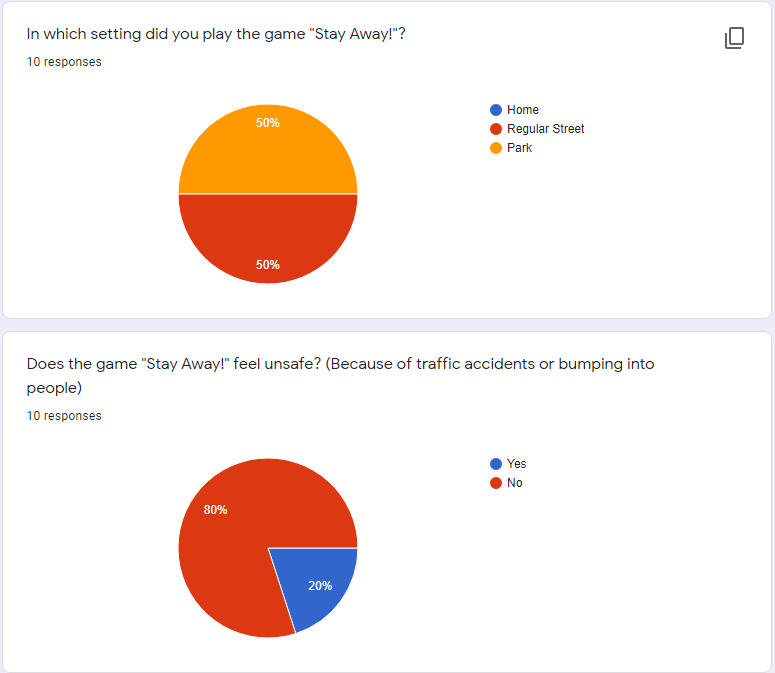
\includegraphics[width = 12cm]{images/unsafe-chart.png}
\caption{This figure shows pie charts provided by the Google Forms website that shows how participants felt about the safety of the application}
\label{fig:unsafe-chart}
\end{figure}

Furthermore, it became evident from the responses that the game wasn't enjoyable or motivating enough to be considered a success. Only one participant rated "Is the game "Stay Away!" a good exercise motivator?" with a 5, and half of participants said the game wasn't enjoyable nor boring; most of the suggestions given by participants were about making the game harder and with faster enemies. With this in mind, some variables were tweaked to make enemies faster and spawning more often, in addition to this, the distance necessary between the player and enemies for the player to take damage was increased.

\section{Summary}
This chapter evaluated the implementation methodologies that were adopted and how they could be improved in a future work. Additionally, the chapter also went through the evaluation methodologies for the application, and how the feedback gathered from these evaluations was used to improve the overall quality of the game.

\chapter{Conclusion}

This paper talked over what the goals and motivations were for this project. The aim was to investigate how location based games work and how making them multiplayer could motivate players to exercise and play together. Requirements set at the beginning of the project were listed to provide an outline, and later in the paper we discussed how they were met and how the application was designed around them. The implementation for various parts of the application was explained in detail followed by an evaluation on how effective these implementation methods were. Additionally, the paper also discussed how the application itself was evaluated and this feedback helped improve the quality. Finally, this chapter will summarize the project and talk about what can be improved or removed in the future works. Lastly, a personal reflection on the subject will be provided.

\section{Summary}

In summary, Stay Away! is a multiplayer Location Based Game that was designed to provide an entertaining experience while also encouraging physical activity. The system uses a host/client network architecture in which a user hosts a temporary server in their devices, and other users connect to that server through that device's IPv4 address. What differentiates this game from other games in the genre (Pokemon GO) is that players are able to see each other's characters in real time, which in turn improves playability. The application's appearance and mechanics have been evaluated by real life participants that later gave feedback by completing a form, this feedback was then used to improve how the game looks and feels, but it's still not a complete project.

The system has proved to be enjoyable as a game but didn't motivate physical exercise in players enough, thus some future changes are planned for this project, which hopefully will bring it closer to envisioned final product.

\section{Future Work}

The future work for "Stay Away!" is mainly focused on adding features that would make it a better exercise motivator. Many features have been planned out that could do such a thing and in this section we will discuss each one of them. The first feature is a calories burned calculator, it has been shown that having user's being able to see how many calories they burned is a good motivator because it helps them determine whether they have met their goals for that session \citep{Sullivan16}. This feature combined with a distance walked counter would be very needed UI additions. Another feature that could improve the motivating factor is a "Goals" tab, in which the user could set out a goal in terms of calories burned and everytime they play the game, the calories burned on that session would be logged and count towards their goal. 

In addition to exercise motivating features, the multiplayer logic can also be improved. The current plan is to change the current host/client logic to a dedicated server one, this would provide various opportunities that aren't possible with current structure, namely an account creation platform; being able to join a lobby from public networks; logging valuable data into a database. This feature has been experienced with as can be seen on \textbf{Figure \ref{fig:server-lobby}}, and AWS offers free space to host a server that can be easily connected to a DynamoDB database.

\section{Personal Reflection}

This project has been extremely helpful to me as it taught me how to manage my time when working with long pieces of work, and also how to properly divide the different workloads in different iterations for more efficiency. Since a lot of the issues faced didn't have a direct answer online, I had to read through large pieces of documentation to be able to fix them, this is a practice that I didn't have before as most of my questions had been asked online before.

In addition to this, I learned a lot about network structures and how to sync data between two or more devices, this will undoubtedly become useful as I plan to work on multiplayer games in the future.

Lastly, this project was the first time I worked with user evaluation even though it is such an important part of application development, and I'm sure I will use the experience I gained from this in future projects.

\begin{appendices}

\chapter{Final Deliverable}

\begin{figure}[H]
\begin{subfigure}[h]{.5\textwidth}
\centering
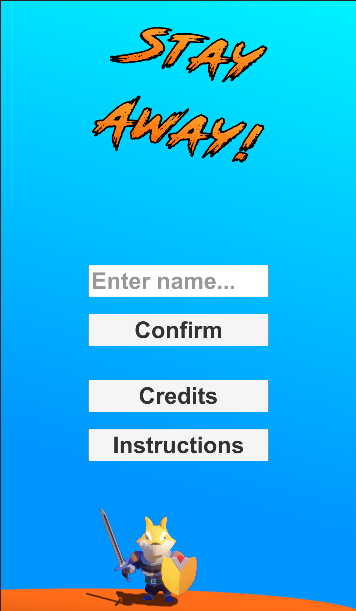
\includegraphics[width = .6\linewidth]{images/final-ui1.png}
\caption{Name selection screen}
\label{fig:f1}
\end{subfigure}
\begin{subfigure}[h]{.5\textwidth}
\centering
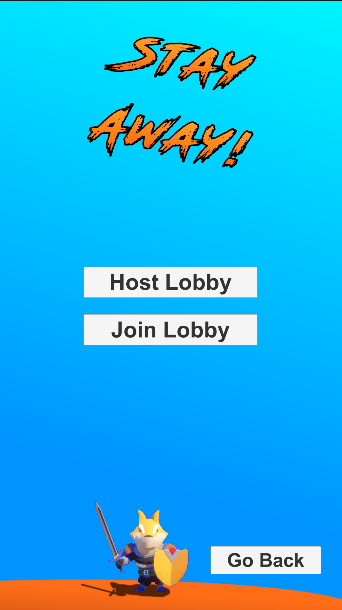
\includegraphics[width = .6\linewidth]{images/final-ui2.png}
\caption{Host/Join lobby screen}
\label{fig:f2}
\end{subfigure}
\begin{subfigure}[h]{.5\textwidth}
\centering
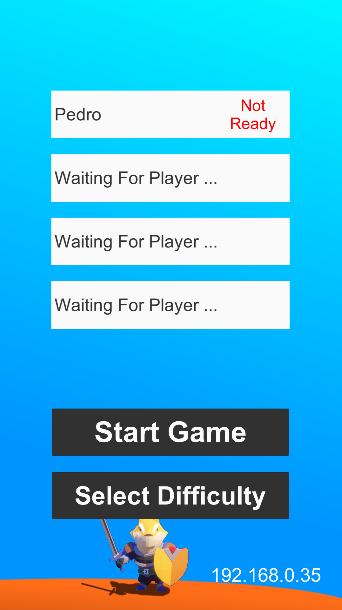
\includegraphics[width = .6\linewidth]{images/final-ui3.png}
\caption{Lobby screen}
\label{fig:f3}
\end{subfigure}
\begin{subfigure}[h]{.5\textwidth}
\centering
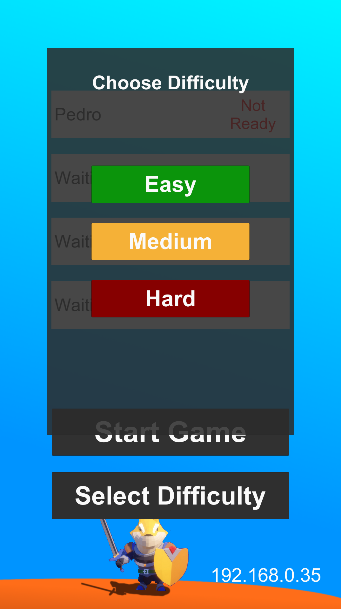
\includegraphics[width = .6\linewidth]{images/final-ui4.png}
\caption{Difficulty screen}
\label{fig:f4}
\end{subfigure}
\caption{Snapshots of the final version of the UI}
\label{fig:final-deliv-ui}
\end{figure}

\begin{figure}[H]
\begin{subfigure}[h]{.5\textwidth}
\centering
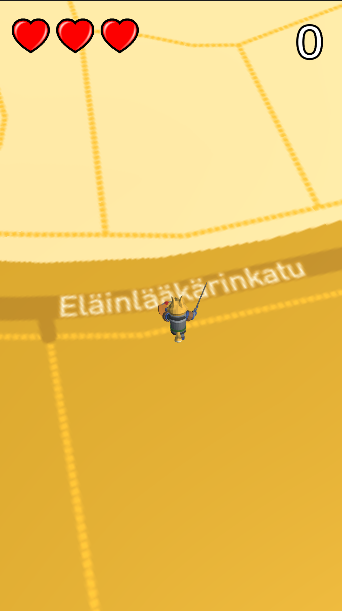
\includegraphics[width = .7\linewidth]{images/final-ui5.png}
\caption{Game screen}
\label{fig:f5}
\end{subfigure}
\begin{subfigure}[h]{.5\textwidth}
\centering
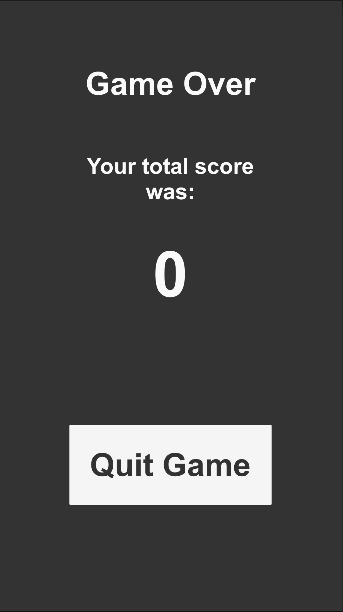
\includegraphics[width = .7\linewidth]{images/final-ui6.png}
\caption{Game Over screen}
\label{fig:f6}
\end{subfigure}
\caption{Snapshots of the final version of the Game}
\label{fig:final-deliv-game}
\end{figure}

\chapter{User Evaluation Forms}

\begin{figure}[H]
\centering
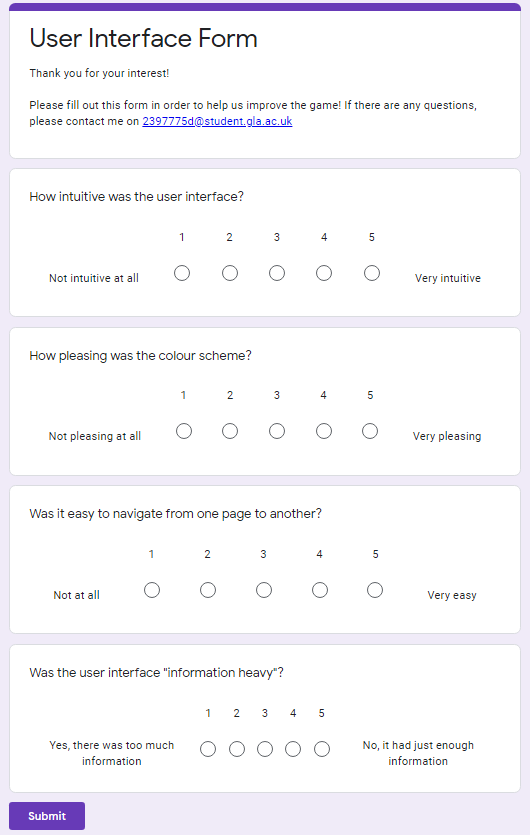
\includegraphics[width = 10cm]{images/ui-form.png}
\caption{Form used to gather feedback on the User Interface}
\label{fig:ui-form}
\end{figure}

\begin{figure}[H]
\centering
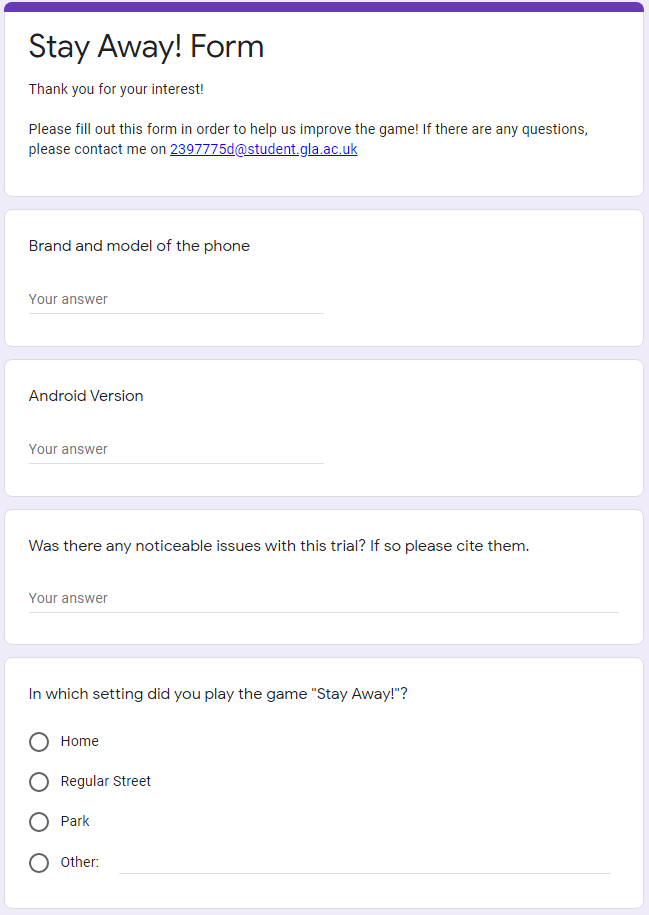
\includegraphics[width = 10cm]{images/game-form1.png}
\caption{First part of the game form}
\label{fig:gf1}
\end{figure}

\begin{figure}[H]
\centering
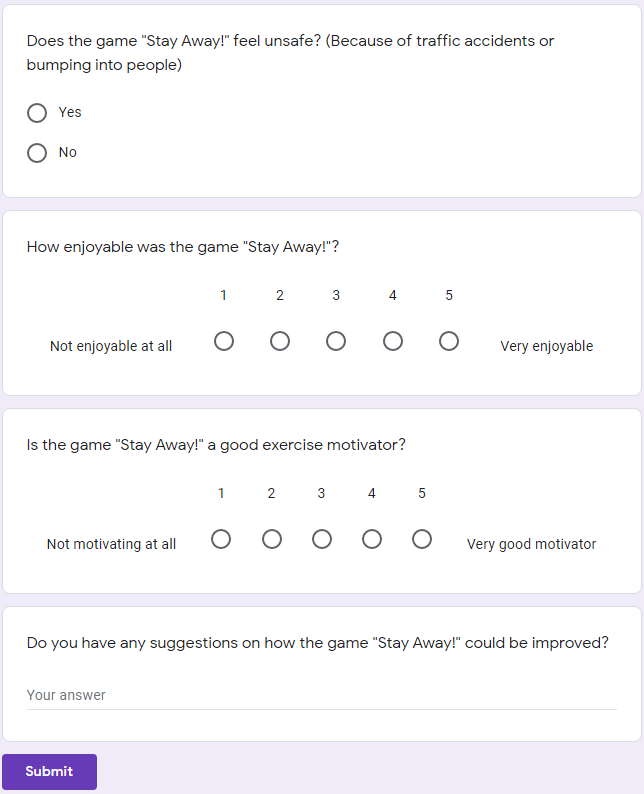
\includegraphics[width = 10cm]{images/game-form2.png}
\caption{Second part of the game form}
\label{fig:gf2}
\end{figure}

\chapter{Instructions and Credit}

\begin{figure}[H]
\centering
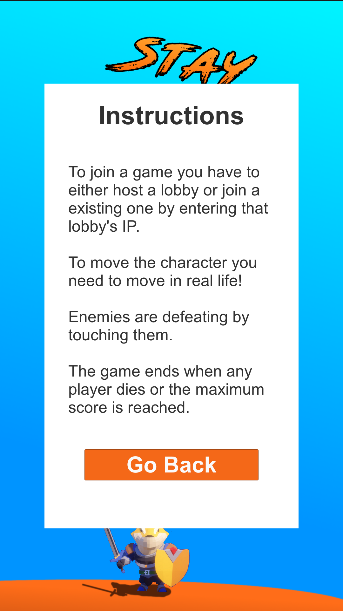
\includegraphics[width = 7cm]{images/final-ui7.png}
\caption{Game Instructions}
\label{fig:f7}
\end{figure}

\begin{figure}[H]
\centering
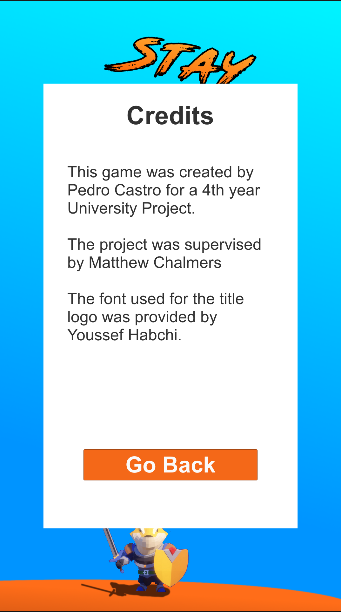
\includegraphics[width = 7cm]{images/final-ui8.png}
\caption{Game Credits}
\label{fig:f7}
\end{figure}

\chapter{Signed Ethics Form}

\begin{figure}[H]
\centering
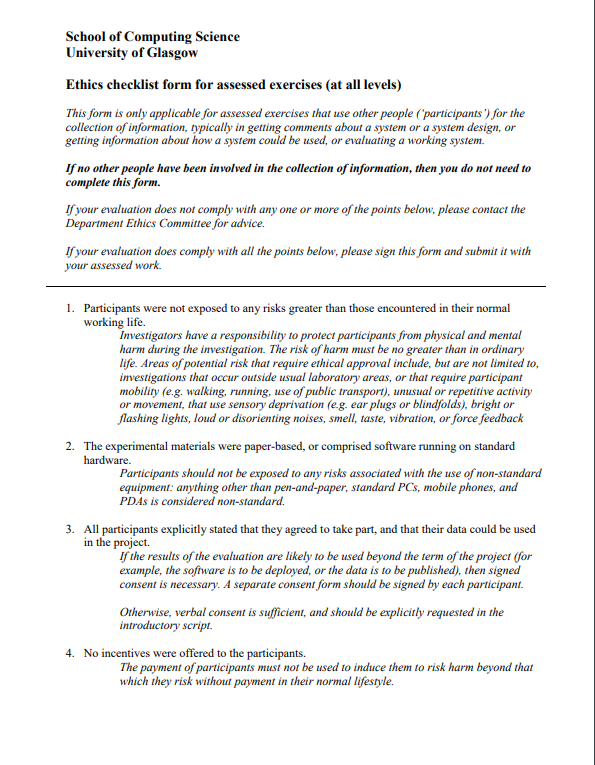
\includegraphics[width = 13cm]{images/signed-form1.png}
\caption{First part of the ethics form}
\label{fig:e1}
\end{figure}

\begin{figure}[H]
\centering
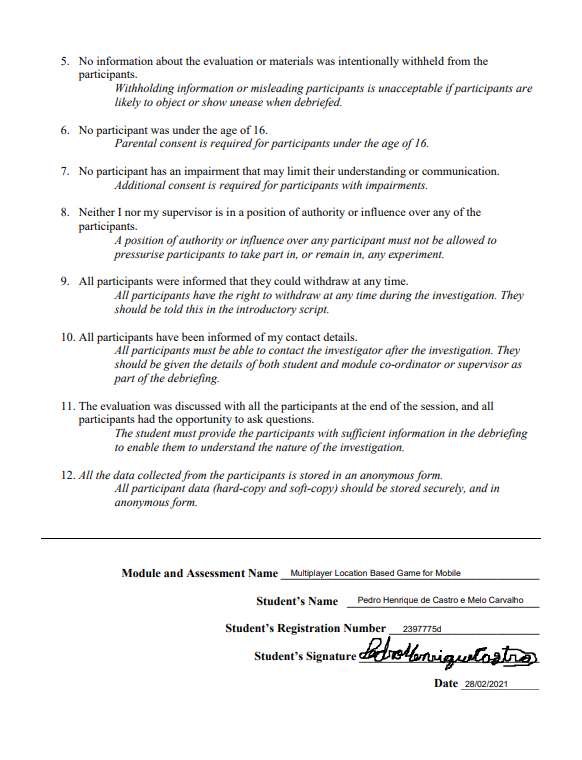
\includegraphics[width = 14cm]{images/signed-form2.png}
\caption{Second part of the ethics form with signature}
\label{fig:e2}
\end{figure}

\end{appendices}

%==============================================================================
%   BIBLIOGRAPHY

\bibliographystyle{abbrvnat}

\bibliography{dissertation}

\end{document}